\anexo{Material suplementar da CGA++}
\label{an:material_cga++}

Este documento é uma referência concisa para a \textit{CGA++}, onde são definidas algumas funções e regras, demonstrando um uso mais avançado e o seu poder expressivo \cite{schwarz2015}.

%Comando para incluir um arquivo em PDF:
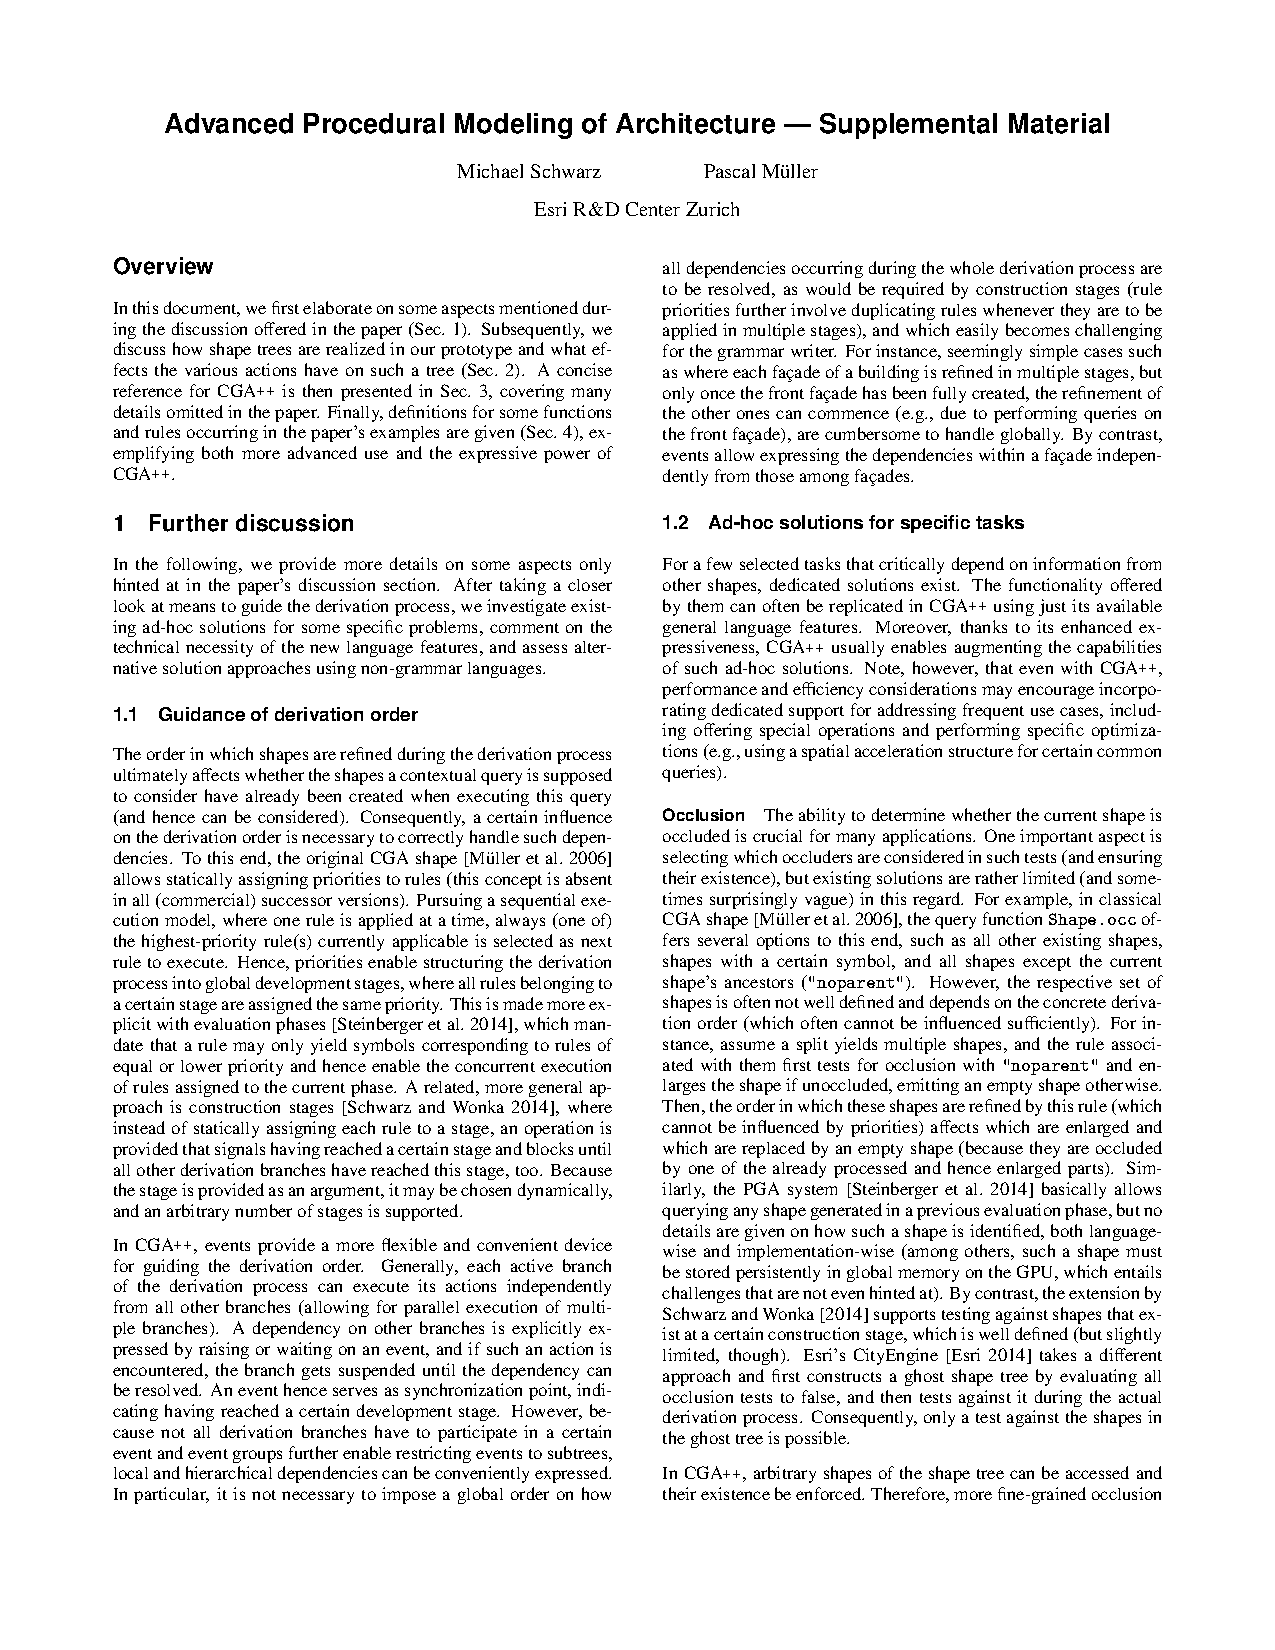
\includepdf[pages={-}]{3-pos-textuais/anexos/cga++_material_suplementar.pdf}